%==========================================================================
%  TRES0312 Fysikk — Foiler-mal
%
%  MØrk/lys modus: kommenter ut én av de to linjene nedenfor.
%==========================================================================
\newif\ifdarkmode
\darkmodetrue      % ← mørk modus
%\darkmodefalse   % ← lys modus  (fjern % foran og legg % foran linjen over)

\documentclass[aspectratio=169, 12pt]{beamer}

\usepackage{amd-beamer}
\usetikzlibrary{overlay-beamer-styles}   % for "visible on=<->" i enkelte tikz-figurer

%--------------------------------------------------------------------------
%  DOKUMENTINFO
%--------------------------------------------------------------------------
\title{Dynamikk}
\subtitle{TRES0312 --- Bevegelsesmengde og Newtons lover}
\author{Ben David Normann}
\date{\today}

%--------------------------------------------------------------------------
%  SEKSJONSKONTEKST
%  \setcounter{section}{N} setter gjeldende seksjonsnummer til N, slik at
%  \defn, \exm og \oppgave får samme nummerering som i kompendiet.
%--------------------------------------------------------------------------
\setcounter{section}{4}   % Kapittel 4: "Dynamikk"

\begin{document}

%--------------------------------------------------------------------------
%  SLIDE 1 — TITTELSIDE
%--------------------------------------------------------------------------
\begin{frame}[plain]
  \titlepage
  \dekkerdelkap{kapittel 4.1--4.2}
\end{frame}

%--------------------------------------------------------------------------
%  SLIDE 2 — Tre kjappe fra forrige gang (sirkelbevegelse, kinematikk)
%--------------------------------------------------------------------------
\begin{frame}{}

  \repetisjon{Tre kjappe fra forrige gang}{%
    \begin{enumerate}[1.]
      \item Hva er formelen for sentripetalakselerasjon, og hvilken retning peker den?
      \item Hvordan kan farten i sirkelbevegelse skrives ved hjelp av omløpstiden $T$?
      \item Hva er sammenhengen mellom sentripetalakselerasjon og omløpstid, $a_\perp = \ldots$?
    \end{enumerate}
  }

\end{frame}

%--------------------------------------------------------------------------
%  SLIDE 3 — Til ettertanke: hva er egentlig en kraft?
%--------------------------------------------------------------------------
\begin{frame}{}

  \tanke{}{%
  ``May the force be with you!'' Takk, men... hva er egentlig en kraft (``force'' på engelsk)?\\[6pt]
  Og: hvorfor er det verre å krasje med en buss som kjører i $5\,\mathrm{km/h}$ enn en flue som flyr i $5\,\mathrm{km/h}$?
  }

\end{frame}

%--------------------------------------------------------------------------
%  SLIDE 4 — Definisjon: Bevegelsesmengde
%--------------------------------------------------------------------------
\begin{frame}{Bevegelsesmengde}

  \defnat{4.1}{Bevegelsesmengde}{
    Bevegelsesmengde, $p$, er definert som produktet av et legemes masse, $m$, og dets hastighet, $v$:
    \[\vec{p} = m \cdot \vec{v}\]
    Enheten for bevegelsesmengde er $\mathrm{kg\cdot m/s}$.
  }

  \pause
  \merk{Vektor}{
  Bevegelsesmengde er en vektor --- den har både størrelse og retning, akkurat som farten $\vec{v}$.
  }

\end{frame}

%--------------------------------------------------------------------------
%  SLIDE 5 — Aktivitet: Ishockey-puck
%--------------------------------------------------------------------------
\begin{frame}{Aktivitet}

  \aktivitet{Ishockey-puck}{%
  En ishockey-puck har masse $m = 170\,\mathrm{g}$ og slås slik at den oppnår farten $v = 40\,\mathrm{m/s}$.
  Hva er bevegelsesmengden til pucken?
  }

\end{frame}

%--------------------------------------------------------------------------
%  SLIDE 6 — Aktivitet: Geværkule og bil
%--------------------------------------------------------------------------
\begin{frame}{Aktivitet}

  \aktivitet{Geværkule og bil}{%
  En typisk geværkule har masse $m_k = 10\,\mathrm{g}$ og forlater løpet med fart $v_k = 900\,\mathrm{m/s}$.
  En bil har masse $m_b = 1500\,\mathrm{kg}$.
  \begin{enumerate}[a)]
      \item Finn bevegelsesmengden til geværkula.
      \item Hvor fort må bilen kjøre for å ha nøyaktig samme bevegelsesmengde som kula?
            Gi svaret i både $\mathrm{m/s}$ og $\mathrm{km/h}$.
  \end{enumerate}
  }

\end{frame}

%--------------------------------------------------------------------------
%  SLIDE 7 — Legeme og kraft som vekselvirkning (Newtons 3. lov)
%--------------------------------------------------------------------------
\begin{frame}{Kraft som vekselvirkning}

  \defnat{4.2}{Legeme}{
  Et legeme er et objekt med masse og posisjon. Massen $m$ måles i kg, og posisjonen $\vec{r}$ måles i meter.
  }

  \pause
  \defnat{4.3}{Kraft som vekselvirkning}{
  En kraft er en vekselvirkning mellom legemer. Krefter opptrer derfor alltid i par: dersom legeme $A$ virker på legeme $B$ med en kraft $\vec{F}$, virker legeme $B$ på legeme $A$ med en kraft $\vec{F}'$, like stor men motsatt rettet:
  \[\vec{F} = -\vec{F}'\qquad\textbf{(Newtons 3. lov)}\]
  }

\end{frame}

%--------------------------------------------------------------------------
%  SLIDE 8 — Figur: kraft og motkraft
%--------------------------------------------------------------------------
\begin{frame}{}

  \begin{figure}[ht!]
  \centering
  \ifdarkmode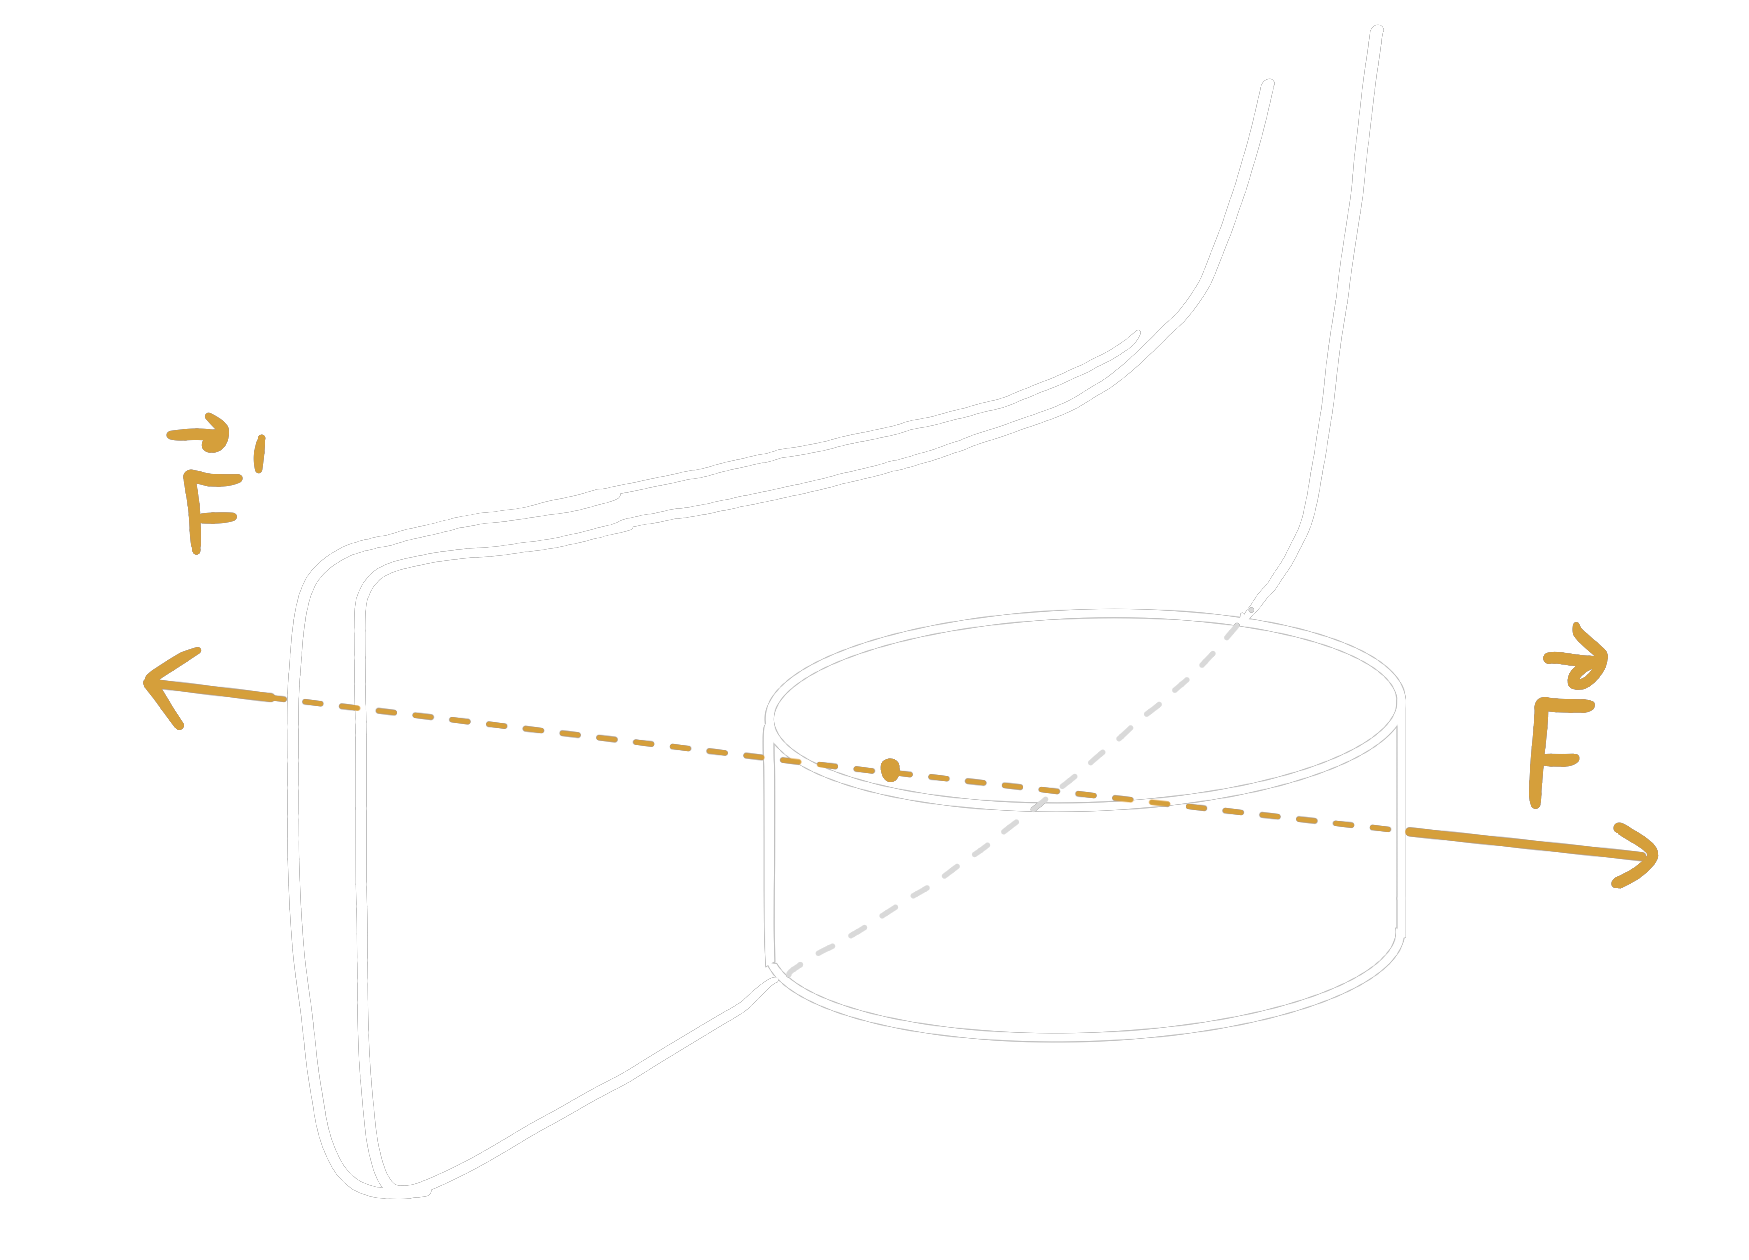
\includegraphics[width=0.62\textwidth]{Images/Kraft_motkraft_mork.png}\else
\includegraphics[width=0.62\textwidth]{Kapittel4:Dynamikk/Kraft_motkraft.png}\fi
  \caption{Kraft er vekselvirkning mellom to legemer, og krefter opptrer derfor alltid i par: kraft og motkraft, som virker på hvert sitt legeme. Disse kreftene er alltid like store og motsatt rettet.}
  \end{figure}

\end{frame}

%--------------------------------------------------------------------------
%  SLIDE 9 — Newtons 2. lov: kraft som endring av bevegelse
%--------------------------------------------------------------------------
\begin{frame}{Newtons 2. lov}

  Fra bevegelsesmengde til kraft: dersom bevegelsesmengden til et legeme endrer seg fra $\vec{p}_1$ til $\vec{p}_2$ i løpet av tiden $\Delta t$, må det ha virket en kraft på legemet.
  \[
    \sum\vec{F} = \frac{\Delta\vec{p}}{\Delta t} = m\frac{\Delta\vec{v}}{\Delta t} = m\vec{a}
  \]

  \pause
  \defnat{4.4}{Kraft som endring av bevegelse}{
  Dersom et legeme blir påvirket av én eller flere krefter, vil legemet akselerere i retning av resultantkraften $\sum\vec{F}$:
  \[
    \sum\vec{F} = m\vec{a}\qquad\textbf{(Newtons 2. lov)}
  \]
  }

\end{frame}

%--------------------------------------------------------------------------
%  SLIDE 10 — Newtons 1. lov: krefter og treghet
%--------------------------------------------------------------------------
\begin{frame}{Newtons 1. lov}

  \tanke{}{%
  Kan et legeme akselerere dersom $\sum\vec{F}=0$?
  }

  \pause
  \defnat{4.5}{Krefter og treghet}{
  Alle legemer har en iboende treghet, kalt \textbf{masse}, som gjør at bevegelsen beholdes så lenge det ikke virker krefter på legemet:
  \[
    \sum\vec{F} = 0 \Leftrightarrow v = \text{konst.}\qquad\textbf{(Newtons 1. lov)}
  \]
  }

\end{frame}

%--------------------------------------------------------------------------
%  SLIDE 11 — Oppsummering: Newtons tre lover
%--------------------------------------------------------------------------
\begin{frame}{}

  \oppsum{Newtons tre lover}{%
  \begin{enumerate}[1.]
    \item[\textbf{1.}] $\sum\vec{F} = 0 \Leftrightarrow v = \text{konst.}$ --- et legeme i ro/konstant fart forblir så, uten ytre krefter.
    \item[\textbf{2.}] $\sum\vec{F} = m\vec{a}$ --- resultantkraften bestemmer akselerasjonen.
    \item[\textbf{3.}] $\vec{F} = -\vec{F}'$ --- krefter opptrer alltid i par (kraft og motkraft).
  \end{enumerate}
  }

\end{frame}

%--------------------------------------------------------------------------
%  SLIDE 12 — Neste gang
%--------------------------------------------------------------------------
\begin{frame}
\begin{center}
  \Huge{Neste gang: Krefter i dagliglivet}
  \begin{itemize}
    \item Kraft fra spiralfjær (Hookes lov)
    \item Tyngdekraft
    \item Underlagskrefter: normalkraft og friksjon
  \end{itemize}
  \vspace{6mm}
  {\normalsize\itshape Kraften er svak i noen av oss, men lovene gjelder alle\ldots}
\end{center}
\end{frame}

\end{document}
